\documentclass[11pt,aspectratio=1610]{beamer}
\usepackage{fbb}
\usetheme{CambridgeUS}
\beamertemplatenavigationsymbolsempty
\usepackage[utf8]{inputenc}
\usepackage{amsmath,adjustbox,mathtools}
\usepackage{amsfonts}
\usepackage{hyperref}
\usepackage{graphicx}
\usepackage{xpatch}
\usepackage{makecell}
\usepackage{tabularx}
\usepackage{csquotes}
\usepackage{adjustbox}
\setbeamertemplate{caption}{\raggedright\insertcaption\par}
\usepackage{minted}
\usetheme{default}
\usecolortheme{default}


% Définition des couleurs
\definecolor{schTag}{RGB}{204, 0, 0}       % Rouge pour les balises
\definecolor{schAttr}{RGB}{0, 0, 153}      % Bleu pour les attributs
\definecolor{schValue}{RGB}{0, 102, 0}     % Vert pour les valeurs
\definecolor{schBg}{RGB}{245, 245, 245}    % Fond gris clair

% Configuration de minted
\setminted{
  bgcolor=schBg,
  frame=single,
  framesep=2mm,
  linenos=true,
  breaklines=true,
  fontsize=\small,
}


\usepackage{pgfplots}
\usepackage{tikz}
\usetikzlibrary{shapes,calc,matrix,decorations.markings,decorations.pathreplacing,positioning, intersections,backgrounds,through,hobby}
\usepackage[english]{babel}
%\AtBeginSection[]
%{\begin{frame}
% \frametitle{}  
%\setlength{\itemsep}{.5cm}
% \tableofcontents[currentsection,
%                  hideothersections,
%		  sectionstyle=hide/hide/hide,
%                  subsectionstyle=show/show/show/hide
%                   ]
% \end{frame} 
% }

%\AtBeginsection[]
%{\begin{frame}
% \frametitle{}  
% \tableofcontents[currentsection,
%	 	  currentsection,
%		  sectionstyle=show/hide,
%                  sectionstyle=show/shaded/hide
%                   ]
% \end{frame} 
% }


\AtBeginSection[]
{
  \begin{frame}
    \tableofcontents[
      currentsection,       % Met en évidence la section courante
      sectionstyle=show/shaded, % Sections : courante en évidence, autres en grisé
      subsectionstyle=hide  % Cache toutes les sous-sections
    ]
  \end{frame}
}
 
 

\AtBeginSubsection[]
{
  \begin{frame}
    \tableofcontents[
     currentsection, % Affiche uniquement la section courante
      hideothersubsections, % Cache les sous-sections des autres sections
      sectionstyle=show/hide, % Cache les autres sections
      subsectionstyle=show/shaded/hide % Sous-section courante en évidence, les autres en grisé
    ]
  \end{frame}
}


\setbeamertemplate{sections/subsections in toc}[square]
\setbeamertemplate{bibliography item}[sqare]
\setbeamertemplate{itemize item}[square]
\setbeamertemplate{enumerate item}[square]
\setbeamertemplate{itemize subitem}[square]




\setbeamertemplate{sections/sections in toc}[square]
\setbeamertemplate{itemize item}[square]
\setbeamertemplate{enumerate item}[square]
\setbeamertemplate{itemize subitem}[square]

\usepackage[style=verbose,citestyle=authoryear,isbn=true,url=false,
doi=true,backend=biber,maxbibnames=9, maxcitenames=4]{biblatex}
\addbibresource{/home/mgl/Bureau/Travail/Communications_et_articles/bibliographie_commune/biblio.bib}
\renewcommand*{\bibfont}{\tiny} 

\usepackage{tikz}
\usetikzlibrary{shapes,calc,matrix,decorations.markings,decorations.pathreplacing,positioning, intersections,backgrounds}
\tikzstyle{bag} = [align=center]

\date[]{}
\author[Matthias \textsc{Gille Levenson}]{\\~\\ Matthias \textsc{Gille Levenson}\\   {\scriptsize Université Versailles Saint Quentin (UVSQ) \& École Normale Supérieure de Lyon, France}\\ {\tiny matthias [dot] gille [-] levenson [at] ens-lyon [dot] fr}\vspace{-1cm}}
\title[TEI schemata]{Introduction générale au XML et à la TEI\\ {\small Atelier Humanités Numériques \& Lyon}}
%\titlegraphic{\hspace{0.5cm}\includegraphics[scale=0.21]{/home/mgl/Bureau/Travail/admin/logos/ensl.png}\hspace{0.5cm}\includegraphics[scale=0.23]{/home/mgl/Bureau/Travail/admin/logos/ciham.pdf}\hspace{0.5cm}}
\usepackage[justification=centering]{caption}
\begin{document}
\maketitle

\section{Introduction}


\begin{frame}{Accès aux slides}
\begin{itemize}
\item \href{https://github.com/matgille/Antidote_workshop_2025_ODD.git}{https://github.com/matgille/Antidote\_workshop\_2025\_ODD.git}
\end{itemize}
\end{frame}

\section{Le format XML}


\begin{frame}{eXtensible Marking Language}
\begin{itemize}
\item XML stands for \textbf{eXtensible Markup Language}.
\item It is a format that allows to describe any kind of textual (or numeric) data 
\item It is the actual \textit{format} the TEI uses, but it might change/evolve in the future.
\end{itemize}
\end{frame}

\begin{frame}{Two important concepts: Conformité and validity}
\begin{itemize}
\item Un document \textbf{doit} être conforme au XML, c'est-à-dire respecter l'ensemble des règles du XML
\item Un document \textbf{peut} être validé par un \textbf{schéma}, c'est-à-dire un document qui vérifie des règles propres à une spécification particulière
\item Quelques spécifications XML: TEI, EAD, DublinCore, AltoXML, PageXML, RDF, etc...
%\item Along with validity comes another important concept/nightmare: \textit{namespaces}. You'll understand soon enough.
\item Nous nous intéresserons à la validité des documents XML dans la seconde session de la formation.
\end{itemize}
\end{frame}


\begin{frame}{Conformité}
\begin{itemize}
\item XML is composed of elements, attributes, attribute values and text.
\end{itemize}
\begin{center}
\begin{figure}
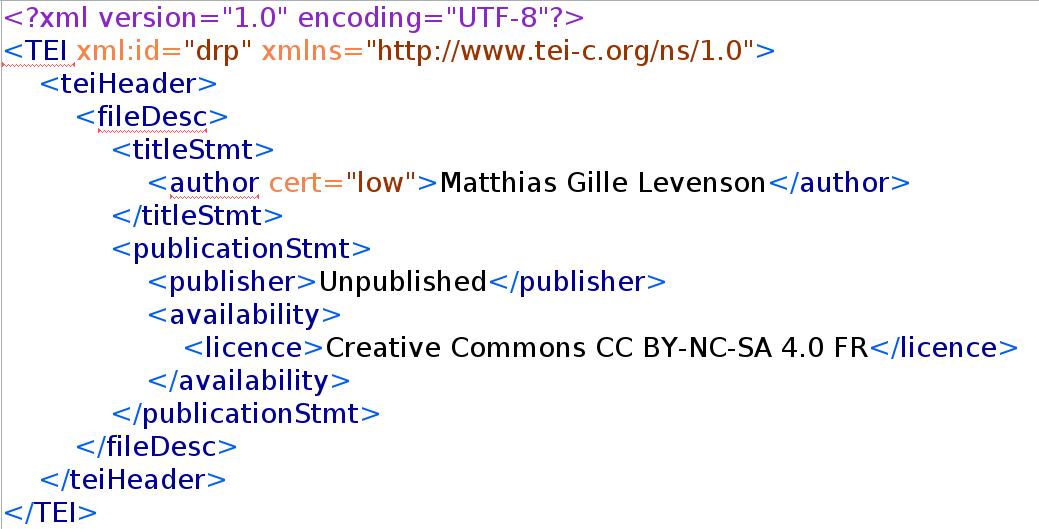
\includegraphics[height=.5\textheight]{img/element_attribute_text.png}
\caption{Ce document XML est conforme (but incorrect/incomplete TEI)}
\end{figure}
\end{center}
%\begin{itemize}
%\item There is little assumption about what can be  in XML (hence eXtensible).
%\end{itemize}
\end{frame}



\begin{frame}{Recap: vocabulary}
Four main objects (called \textit{nodes}):
\begin{itemize}
\item \textbf{Element} nodes: the basic object of any XML document: \\ \texttt{<elementName/>} or \texttt{<elementName>...</elementName>}
\item \textbf{Attribute} nodes: part of an element that helps specifying it: \\ \texttt{attributeName="value"}
\item \textbf{Text nodes}: every textual object inside an element
\item \textbf{Comment} nodes: content not parsed by the machine: \\ \texttt{<!-{}- some useful comment -{}->}
\end{itemize}
\end{frame}


\begin{frame}{The root node/element}
\begin{itemize}
\item One and only one top element that contains everything else
\end{itemize}
\begin{center}
\begin{figure}
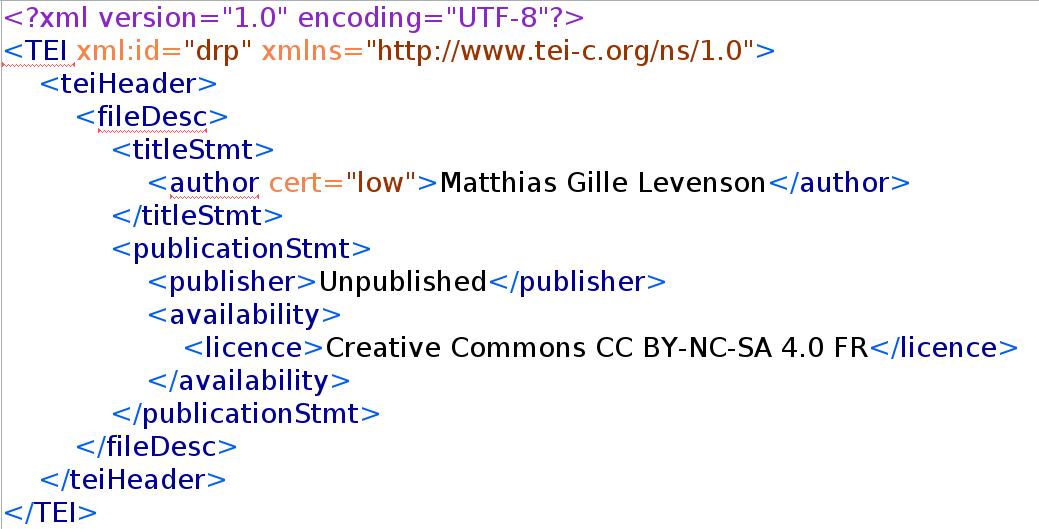
\includegraphics[height=.5\textheight]{img/element_attribute_text.png}
\caption{Ce document XML est \textbf{conforme} (mais la TEI est \textbf{invalide})}
\end{figure}
\end{center}
\end{frame}


\begin{frame}{Conformité}
\begin{itemize}
\item \textit{No} overlapping elements
\end{itemize}
\begin{center}
\begin{figure}
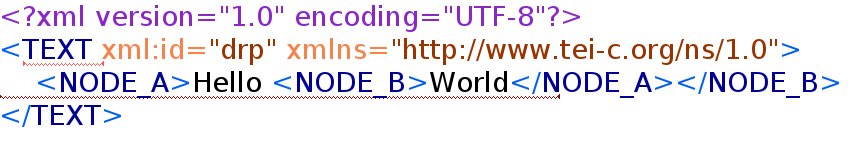
\includegraphics[width=.9\textwidth]{img/overlapping.png}
\caption{Ce document XML est non conforme}
\end{figure}
\end{center}
\end{frame}


\begin{frame}{Conformité}
\begin{itemize}
\item Some elements can contain other elements, but elements can also be empty
\end{itemize}
\begin{center}
\begin{figure}
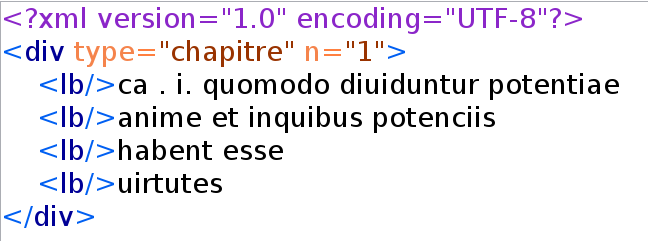
\includegraphics[width=.9\textwidth]{img/empty.png}
\caption{Ce document XML est conforme}
\end{figure}
\end{center}
\end{frame}



\begin{frame}{Conformité}
\begin{itemize}
\item Les valeurs d'attributs vont entre guillemets
\end{itemize}
\begin{center}
\begin{figure}
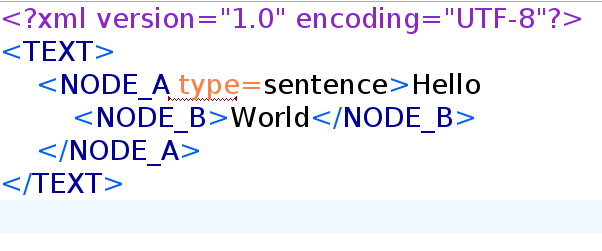
\includegraphics[height=.5\textheight]{img/attributes.png}
\caption{Ce document XML est non conforme}
\end{figure}
\end{center}
\end{frame}



\begin{frame}{Conforme? Non conforme?}
\begin{center}
\begin{figure}
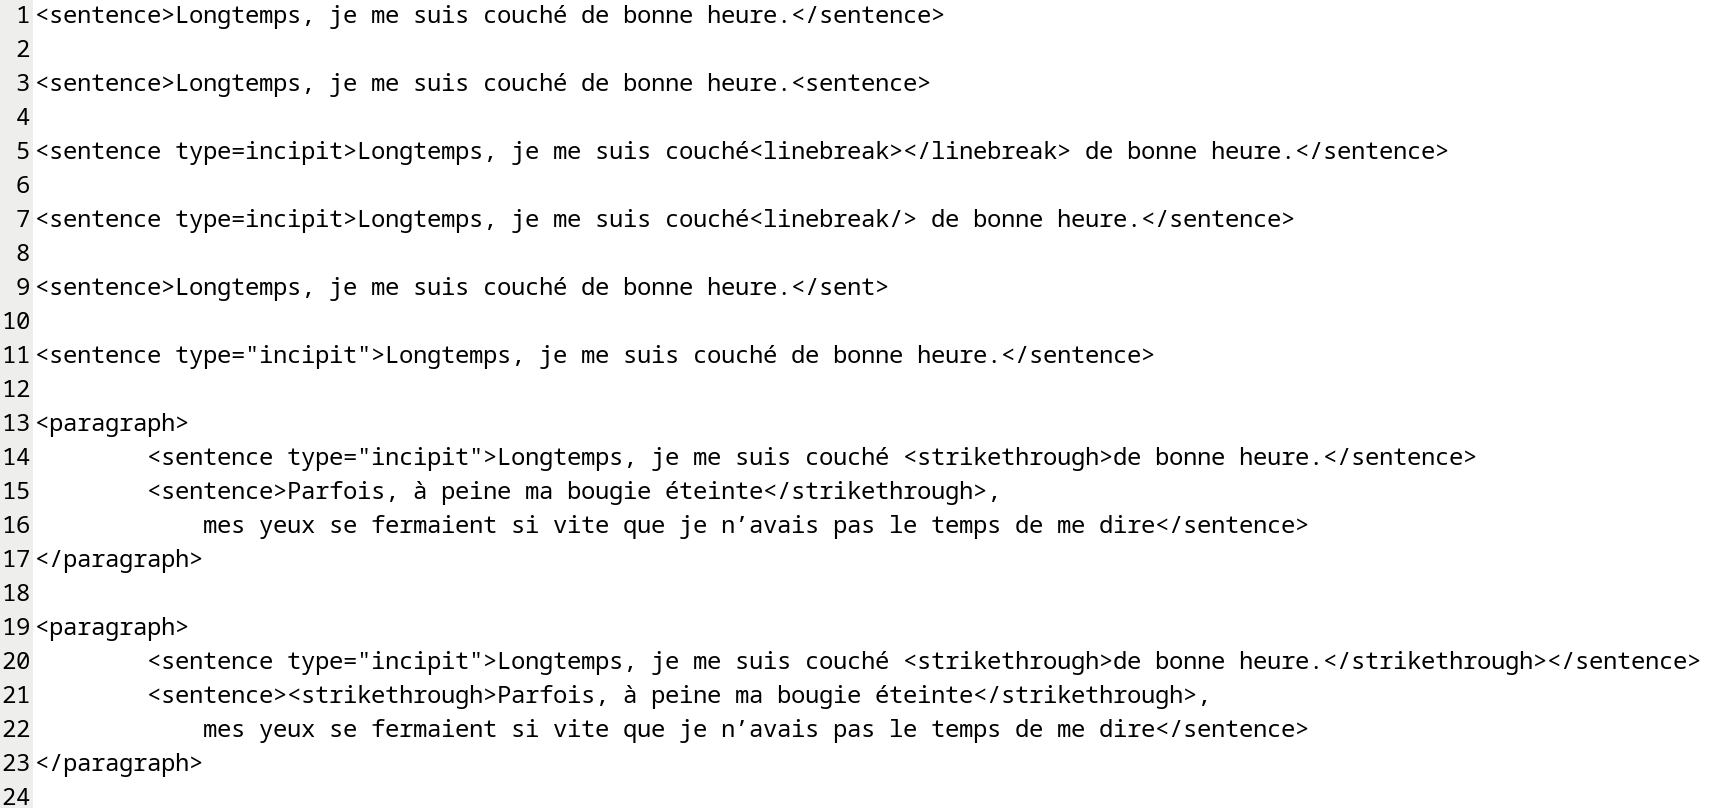
\includegraphics[height=.8\textheight]{img/conformant.png}
\end{figure}
\end{center}
\end{frame}



\section{Qu'est-ce que la TEI?}

\subsection{Ce qu'est la TEI}
\begin{frame}{Qu'est-ce que la TEI?}
\begin{itemize}
\item Une communauté scientifique
\item Une \enquote{standard} et un ensemble de règles, les \textit{Guidelines}: \url{https://tei-c.org/release/doc/tei-p5-doc/en/html/}
\item Une façon de se représenter / modéliser \enquote{le} texte
\end{itemize}
\end{frame}


\subsection{Ce que n'est pas la TEI}


\begin{frame}{Ce que n'est pas la TEI}
\begin{itemize}
\item Un outil de visualisation des sources textuelles
\item Un outil de transformation des sources textuelles
\end{itemize}
\end{frame}


\subsection{Principes}
\begin{frame}{}
\begin{itemize}
\item Separate the appearance and the \enquote{essence} of textual objects
\end{itemize}
\begin{center}
\begin{figure}
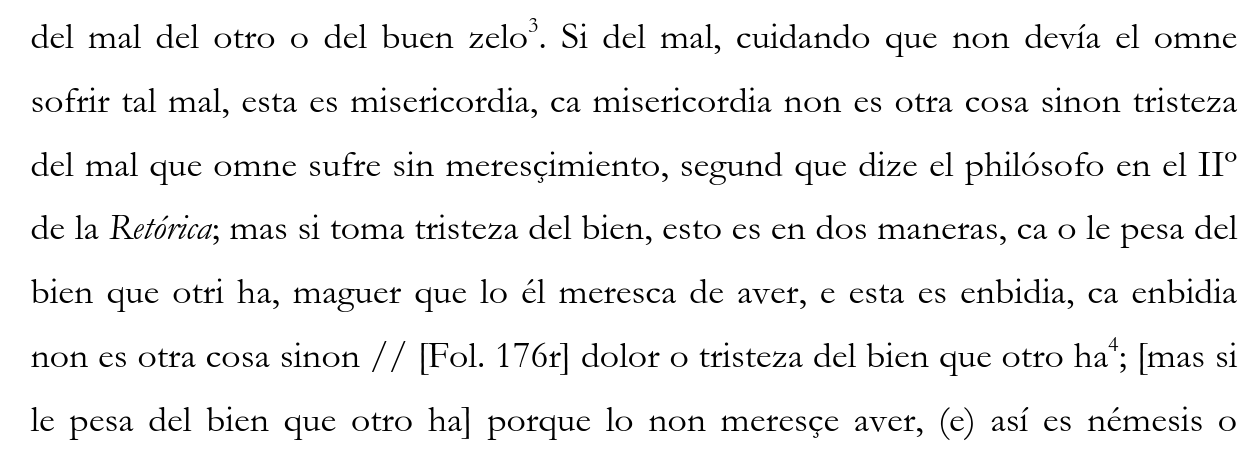
\includegraphics[width=.8\textwidth]{img/texte.png}
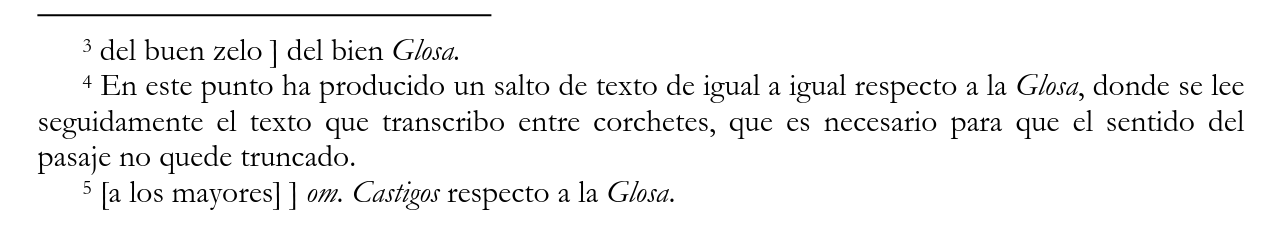
\includegraphics[width=.8\textwidth]{img/apparat.png}
\caption{Fragment of an edition of the \textit{Castigos de Sancho IV} \parencite{sanchez_VersionInterpoladaCastigos_2003}}
\end{figure}
\end{center}
\end{frame}

\begin{frame}{}
\begin{itemize}
\item Séparer l'apparence et l'\enquote{essence} des objets textuels
\end{itemize}
\begin{center}
\begin{figure}
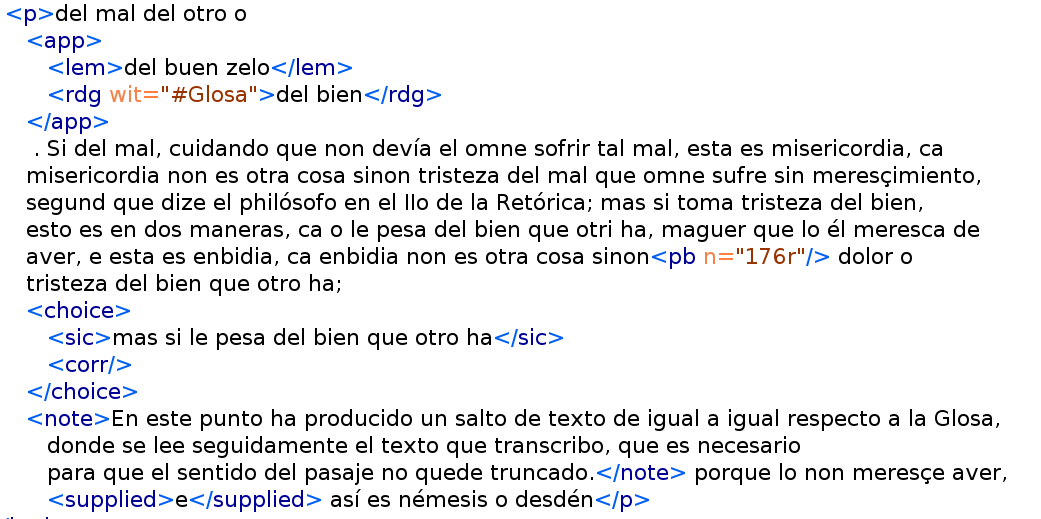
\includegraphics[width=.8\textwidth]{img/xml_structured.png}
\caption{Its possible representation in XML-TEI}
\end{figure}
\end{center}
\end{frame}


\section{La TEI, pour quoi faire?}
\begin{frame}{La TEI, pour quoi faire?}
\begin{itemize}
\item Describing a text using the experience of a \textbf{large community}
\item Producing semantic data that can be \textbf{read} by the human and \textbf{processed} by the computer
\item Make sharing and reusability of these representations easier
\end{itemize}
\end{frame}



\subsection{Décrire des textes / traiter des représentations textuelles}

\begin{frame}{Un exemple de traitement du texte: la collation automatisée}
\begin{minted}{python}
For rdg in apps:
    if rdg.is_empty():
        if preceding_rdg.is_empty():
            create_node(witEnd)
\end{minted}
\end{frame}


\section{Projets utilisant la TEI}




\begin{frame}{References}
\printbibliography
\end{frame}

\end{document}
